\subsection{Setup}

This section now explores how implementing a block based VTAGE value predictor improves the performance of core composition, with and without the new block fetching scheme.
Once again, four configurations are explored:
\begin{itemize}
\item Normal fetching scheme with no value prediction (\novp).
\vspace{-1em}
\item Normal fetching scheme with VTAGE value prediction (\vt).
\vspace{-1em}
\item New fetching scheme with no value prediction (\nfnovp).
\vspace{-1em}
\item New fetching scheme with VTAGE value prediction (\nfvt).
\end{itemize}
The objective of this section is to demonstrate that current work in value prediction can be used to improve the performance of large core compositions, and to show the difference between a real predictor and a perfect predictor.


\begin{table}[t]
  \small
  \centering
 \begin{tabular} {| l | l | l | l | l | l | }
 \hline
    & \cellcolor[gray]{0.7}Disparity & \cellcolor[gray]{0.7} Localization& \cellcolor[gray]{0.7} MSER& \cellcolor[gray]{0.7} Multi\_NCut& \cellcolor[gray]{0.7} Sift\\ \hline
 \vt   & 16  & 16 & 4  & 16& 16\\ \hline
 \nfvt   & 16  & 16 & 4  & 16& 16\\ \hline
	  & \cellcolor[gray]{0.7} Stitch & \cellcolor[gray]{0.7} SVM & \cellcolor[gray]{0.7} Text. Synth & \cellcolor[gray]{0.7} Tracking&\\ \hline
   \vt & 16  & 16 & 4  & 16 & \\ \hline
 \nfvt   & 16  & 16 & 4  & 16 &\\ \hline

	\end{tabular}
  \caption{Number of cores composed given a configuration.}\label{tab:conf_cores}
  \vspace{1em}
\end{table}


\subsection{Results}
\begin{figure}[t]
    \centering
    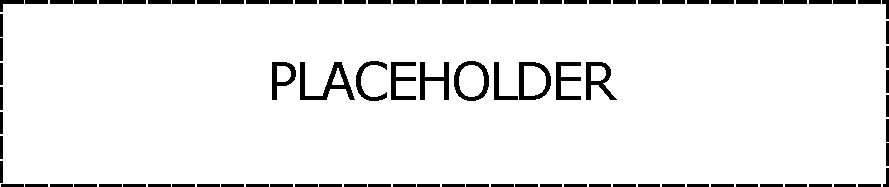
\includegraphics[width=1\textwidth]{chapter3/graphics/wip.pdf}
    \caption{Comparing the performance of the standard fetching scheme to the new fetching scheme, with and without perfect value prediction. Higher is better.}
    \label{fig:vtag_perf}
	\vspace{1em}
\end{figure}

\paragraph*{VTAGE Accuracy}
\begin{figure}[t]
    \centering
    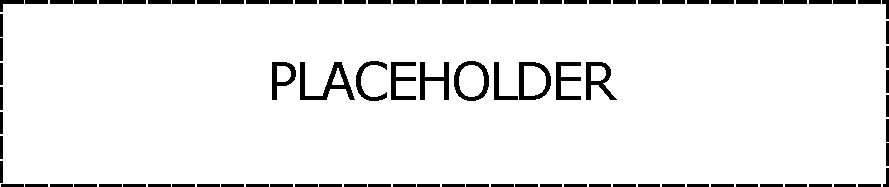
\includegraphics[width=1\textwidth]{chapter3/graphics/wip.pdf}
    \caption{Comparing the performance of the standard fetching scheme to the new fetching scheme, with and without perfect value prediction. Higher is better.}
    \label{fig:vtag_accuracy}
	\vspace{1em}
\end{figure}